\chapter{Magnetoestática}


\section{Corriente y densidad de corriente}

Cuando existen cargas en movimiento, se define la \textit{corriente eléctrica} $I$ como
la cantidad de \textit{carga neta} que pasa por unidad de tiempo a través de una superficie $S$ \textit{en una dirección determinada}, 
\begin{equation}\marginnote{Corriente eléctrica}
I(t) :=\lim_{\Delta t\to 0}\frac{\Delta Q}{\Delta t}=\frac{dQ}{dt},
\end{equation}
de modo que la carga neta que atraviesa entre los tiempos $t_1$ y $t_2$ una superficie por donde circula una corriente $I(t)$ es
\begin{equation}
Q=\int_{t_1}^{t_2}I(t)\,dt.
\end{equation}
La unidad S.I. para la corriente es el \textbf{Amp\`ere}: $1A:=1C/1s$.

\subsection{Densidad de Corriente}

Consideremos una superficie sobre la cual inciden cargas con densidad $\rho$,
moviéndose con velocidad $\vec{v}$, cruzando un elemento de superficie (orientado) $d\vec{S}$.
\begin{figure}[!h]
\centerline{\includegraphics[height=4cm]{fig/fig-flujo-cargas-01.pdf}}
\caption{Carga con densidad $\rho$ flujendo con velocidad $\vec{v}$ a través
de un elemento de superficie $d\vec{S}$.}
\label{MD1}
\end{figure}
La carga neta que atraviesa el área $dS$ en un intervalo de tiempo $dt$ es la que
está contenida en un cilindro oblicuo de base $dS$ y de largo $v\,dt$. Ver
figura \ref{MD1}.

Esto permite escribir:
\begin{equation}
dQ=\rho\, dV=\rho\, dS\,(v\,dt)\cos\theta=\rho\,\vec{v}\cdot d\vec{S}\,dt.
\end{equation}
Definimos la \textbf{densidad de corriente}
\begin{equation}\marginnote{Densidad de Corriente}
\boxed{\vec{J}(x):=\rho(x)\vec{v}(x),}
\end{equation}
de modo que
\begin{equation}
 dQ=\vec{J}\cdot d\vec{S}\,dt .
\end{equation}
En otras palabras, la densidad de corriente es la carga por unidad de tiempo y
por unidad de superficie que atraviesa un elemento de área normal dado.
Como consecuencia, la corriente, es decir, la carga por unidad de tiempo,
que atraviesa una superficie $S$ es dada por
\begin{equation}
I=\int_{S}\vec{J}\cdot d\vec{S}.
\end{equation}
Es importante notar que si $\rho>0$, entonces $\vec{J}$ y $\vec{v}$ tienen igual
sentido, mientras que si $\rho<0$, entonces $\vec{J}$ y $\vec{v}$ tienen
sentidos opuestos.

\section{Conservación de la carga eléctrica}

La ley (experimental) de conservación (local) de la carga eléctrica puede ser escrita
en general, como
\begin{equation}
\frac{d{\ }}{dt}\int_V \rho\,dV=-\int_{\partial V}\vec{J}\cdot d\vec{S},
\end{equation}
que expresa el hecho que todo cambio en la carga neta contenida en un volumen $V$ dado (pero arbitrario) es debido al flujo neto de carga por la superficie ${\partial V}$ que lo encierra. Usando el teorema de Gauss, podemos transformar la integral de superficie a una integral de volumen, obteniendo
\begin{equation}
\int_V\left(\frac{\partial\rho}{\partial t}+\vec{\nabla}\cdot\vec{J}\right)\,dV
 =0.
\end{equation}
Como esta relación debe ser válida para todo volumen $V$, es decir, de tamaño y forma arbitraria, es necesario que
\begin{equation}\marginnote{Conservación local carga}
\boxed{\frac{\partial\rho}{\partial t}
+\vec{\nabla}\cdot\vec{J}=0.}\label{eccont}
\end{equation}
Esta relación es conocida como la \textit{ecuación de continuidad}.

\subsection{Corrientes Estacionarias}

Un caso de particular interés es aquel en que las corrientes son
\textit{estacionarias}, es decir, en las que tanto $\rho$ como $\vec{J}$ \textit{no dependen del tiempo}. Bajo estas condiciones, la ecuación de continuidad requiere que la
divergencia de la densidad de corriente sea nula:
\begin{equation}\marginnote{Caso estacionario}
 \vec{\nabla}\cdot\vec{J}=0. \label{divJ0}
\end{equation}


% \subsection{Modelo de Conductividad}
%
% Suponemos que los electrones se mueven en la red atómica. La ecuación
% de movimiento es
% \begin{equation}
% mn\frac{du_i}{dt} -nqE_i=F_i%
% \label{magstatica-mov}%
% \end{equation}
% donde $T$ es la temperatura del gas de electrones, y $F_i=-mn\nu u_i$ es
% la fuerza debido a las colisiones. Recordando que $\rho=nq$ y que
% $j_i=nqu_i$ tenemos que en la ecuación (\ref{eccont} )
% resulta%
% \begin{equation}
% \frac{\partial\rho}{\partial t}+\partial_i\left(  \rho u_i\right)  =0
% \end{equation}
% de la ecuación (\ref{magstatica-mov}) y suponiendo que el gradiente de
% temperatura es despreciable, tenemos%
% \begin{align*}
% mn\frac{du_i}{dt}-nqE_i  & =-mn\nu u_i\\
% n\frac{d\left(  u_i\right)  }{dt}  & =\frac{nq}{m}E_i-\nu u_i%
% \qquad\qquad/\cdot q\\
% \frac{d\left(  nqu_i\right)  }{dt}  & =\frac{nq^2}{m}E_i-\nu nqu_i\\
% \frac{dj_i}{dt}+\nu j_i  & =\frac{nq^2}{m}E_i%
% \end{align*}
% Si $\vec{J}$ es constante en el tiempo%
% \begin{equation}
% j_i=\frac{nq^2}{m\nu}E_i=\sigma E_i%
% \end{equation}
% llamando a $\sigma$ conductividad eléctrica. Notar que la conductividad es
% inverso a la resistencia eléctrica, es decir, $\sigma=1/R~~\left[
% 1/\Omega\right]  $

% \subsubsection{Aplicación: Velocidad de distribución de la carga}
%
% Velocidad con que se distribuye la carga eléctrica en un conductor con
% conductividad $\sigma$. Veamos que,%
% \begin{equation}
% j_i=\sigma E_i%
% \end{equation}
% luego en la euación de continuidad (\ref{eccont} ) tenemos%
% \begin{align*}
% \frac{\partial\rho}{\partial t}+\vec{\nabla}\cdot\vec{J}  & =0\\
% \frac{\partial\rho}{\partial t}+\sigma\partial_iE_i  & =0\\
% \frac{\partial\rho}{\partial t}+\frac{\sigma}{\varepsilon_0}\rho & =0
% \end{align*}
% Esta ecuación diferencial tiene como solución%
% \begin{equation}
% \rho(t)=\rho_0~e^{-t/t_0}%
% \end{equation}
% donde $t_0=\varepsilon_0/\sigma$. Para valores experimentales tenemos que
% $\varepsilon_0=8.8512\times10^{-12}~\left[  c^2/Nm^2\right]  $ y para el
% cobre se tiene que $\sigma=59.88~\left[  1/\Omega\right]  $ luego conociendo
% la densidad del cobre podemos saber como varia la densidad de carga en el
% tiempo para un volumen dado.

\section{Campo magnético y fuerza magnética}
Se ha encontrado \textit{experimentalmente} que la fuerza que actúa sobre una pequeña carga $q$, moviéndose con velocidad $\vec{v}$ en un campo magnético dado es proporcional a $q$, a la rapidez $v$, y que tiene dirección perpendicular a $\vec{v}$. Esto permite \textit{definir}  la \textit{intensidad de campo magnético} $\vec{B}$ como un (pseudo-)vector tal que (en el sistema internacional de unidades)
\begin{equation}
 \vec{F}_{\rm m}=q\,\vec{v}\times\vec{B}.
\end{equation}
Por lo tanto, la fuerza total que actúa sobre una carga $q$ en un punto del espacio con campo eléctrico $\vec{E}$ y magnético $\vec{B}$ es dada por la \textit{fuerza de Lorentz}\footnote{En honor a Hendrik Antoon Lorentz (1853-1928): físico y matemático holandés. Ganador del Premio Nobel de Física en 1902. Ver \url{http://es.wikipedia.org/wiki/Hendrik_Lorentz}.}
\begin{equation}\marginnote{Fuerza de Lorentz}
\boxed{ \vec{F}=q\left(\vec{E}+\vec{v}\times\vec{B}\right).}
\end{equation}
La unidad de medida de la intensidad de campo magnético $\vec{B}$ es entonces  $[B]=Ns/Cm=Vs/m^2$ , que se define como un \textit{Tesla}: $1T:=Vs/m^2$. Alternativamente se define un
\textit{Gauss} como $1G:=10^{-4}T$. \footnote{Por ejemplo, la magnitud campo
magnético interestelar oscila entre $0.1$ and $10$ $nT$, el campo magnético
de la Tierra es de orden $\approx 0.5 G$, mientras que un imán
de Neodimio (Nd${}_2$Fe${}_{14}$B) produce un campo del orden de $1.25\, T$.
El magneto de un típico sistema de imágen por resonancia magnética (MRI) produce campos entre $1.5\,T$ y $3\,T$. El sistema MRI con el mayor campo magnético construido (mayor resolución) tiene un campo de $11,7\,T$. Los campos magnéticos estables más intensos producidos en un laboratorio son del orden de $45\,T$, mientras que el récord mundial es de $1200\,T$ \cite{Brecord2018} para campos de (muy) corta duración (del orden de los microsegundos). El campo magnético en una estrella de neutrones puede oscilar entre $1$ y $100\, MT$.}

Como consecuencia directa del hecho que la fuerza magnética es perpendicular a
la velocidad de las cargas, \textit{el campo magnético no realiza trabajo} sobre ellas.
Esto tiene como consecuencia que el campo magnético sólo puede cambiar la
dirección de la velocidad de una carga y no su módulo (energía cinética).

Si las cargas están distribuidas continuamente, entonces la fuerza magnética total sobre una región $V$ con densidad $\rho$ y velocidad $\vec{v}$ será
\begin{equation}\marginnote{Fuerza magnética}
 \vec{F}_{\rm m}=\int_V
\rho\vec{v}\times\vec{B}\,dV=\int_V\vec{J}\times\vec{B}\,dV. \label{fm1}
\end{equation}
Podemos describir esta situación usando la \textbf{densidad de fuerza
magnética} $\vec{f}_{\rm m}$, definida como la fuerza por unidad de volumen,
dada por
\begin{equation}
 \vec{f}_{\rm m}:=\vec{J}\times\vec{B},
\end{equation}
de modo que
 \begin{equation}
\vec{F}_{\rm m}=\int_V\vec{f}_{\rm m}\,dV. \label{dfm}
\end{equation}


% \subsection{Trayectorias en un campo eléctromagnético}
% Usando () y la segunda ley de Newton, tenemos
% \begin{equation}
% m\frac{dv_i}{dt}=qE_i+q\varepsilon_{ijk}v_jB_k
% \end{equation}
% Multiplicando esta ecuación con $v_i$, obtenemos
% \begin{equation}
%  \frac{d\ }{dt}(\frac{m}{2}v^2)=qv_iE_i
% \end{equation}
% \begin{equation}
%  \frac{dK}{dt}=qv_iE_i
% \end{equation}
% Sólo el campo eléctrico realiza trabajo sobre la carga, modificando su
% energía cinética.
% \begin{equation}
%  dK=qv_iE_idt=qE_idx_i=-q\partial_i\phi dx_i=-qd\phi
% \end{equation}
% \begin{equation}
%  d(K+q\phi)=0
% \end{equation}
% \begin{equation}
%  \frac{1}{2}mv^2+q\phi={\rm cte}
% \end{equation}
% a lo largo de la trayectoria.


\section{Ley de Biot-Savart}
Biot\footnote{Jean Baptiste Biot: Físico, Astrónomo y Matemático francés (1774-1862). Ver \url{http://es.wikipedia.org/wiki/Jean_Baptiste_Biot}.} y Savart\footnote{Félix Savart: Físico, Médico y Profesor francés (1791-1841). Ver \url{http://es.wikipedia.org/wiki/F\%C3\%A9lix_Savart}.} encontraron ($\sim$\,1820) que el campo magnético $d\vec{B}$ que un pequeño segmento $dx'$ orientado en la dirección de flujo de la corriente $I$ y ubicado en la posición $\vec{x}'$ produce en un punto de posición $\vec{x}$ es proporcional a la intensidad de corriente, al largo del
pequeño segmento, e inversamente proporcional al cuadrado de la distancia
entre el segmento y el punto de observación, es decir,
\begin{equation}
 \left\vert d\vec{B}\right\vert \propto
\left(I,dx',\frac{1}{\left|\vec{x}-\vec{x}'\right|^2}\right),
\end{equation}
y que la dirección del campo producido es perpendicular a $d\vec{x}'$ y al
vector que une el segmento con el punto de observación,
\begin{equation}
d\vec{B}  \perp\left(  d\vec{x}', \vec{x}-\vec{x}' \right) ,
\end{equation}
y que, finalmente, el sentido del campo magnético es dado por la regla de la mano derecha a partir de los vectores $d\vec{x}'$ y $\vec{x}-\vec{x}'$. Ver figura \ref{fBS1}. 
\begin{figure}[!h]
\centerline{\includegraphics[height=6cm]{fig/fig-Biot-Savart-01.pdf}}
\label{Esquema para la ley de Biot-Savart.}
\label{fBS1}
\caption{Ley de Biot-Savart.}
\end{figure}
En resumen,
\begin{equation}
dB_i=kI\varepsilon_{ijk}dx'_j\frac{\left(x_k-x'_k\right)}{\left\vert
\vec{x}-\vec{x}'\right\vert^3},
\end{equation}
donde $k$ es una constante, que depende del sistema de unidades usado y que,
en el Sistema Internacional, \textit{se define} como
\begin{equation}
k=\frac{\mu_0}{4\pi}=10^{-7}~\left[  \frac{V\,s}{A\,m}\right],
\end{equation}
y donde $\mu_0$ es llamada la constante de \textbf{permeabilidad magnética del vacío}.

Con esto, escribimos la \textbf{ley de Biot-Savart} como
\begin{equation}
dB_i=\frac{\mu_0}{4\pi}I\,\varepsilon_{ijk}dx'_j\frac{\left(x_k-x'_k\right)}
{\left\vert \vec{x}-\vec{x}'\right\vert ^3}.
\end{equation}
Usando el \textbf{principio de superposición} obtenemos una expresión para el campo producido por un cable de longitud finita, pero muy delgado:
\begin{equation}
\boxed{B_i(x)=\frac{\mu_0}{4\pi}\int_{\cal C}\varepsilon_{ijk}Idx'_j
\frac{\left(x_k-x'_k\right)}{\left\vert\vec{x}-\vec{x}'\right\vert^3}.}
\label{BS1}
\end{equation}

Podemos generalizar este resultado al caso de una distribución volumétrica de corriente, descrita por su densidad de corriente. Para esto, consideramos un pequeño ``tubo de corriente"\, de sección transversal $dS$ que sigue las líneas de flujo, es decir, tal que el vector normal a la superficie transversal, $\hat{n}$, es paralalo a $\vec{J}$. Entonces, $\vec{J}=J\hat{n}$, $d\vec{x}=d\ell\,\hat{n}$, y además $dV=d\ell\, dS$ (ver figura \ref{fig:tc}), de modo que podemos escribir
\begin{equation}
I\, d\vec{x}=(J dS)(\hat{n}d\ell)=(J\hat{n})(d\ell dS)=\vec{J}\,dV.
\end{equation}
\begin{figure}[!h]
\centerline{\includegraphics[height=4cm]{fig/fig-tubo-de-corriente.pdf}}
\caption{Una distribución volumétrica y los ``tubos de corriente'' asociados.}
\label{fig:tc}
\end{figure}
Con esto podemos encontrar la forma general que usaremos para la ley de Biot-Savart:
\begin{equation}\marginnote{Ley de Biot-Savart}
 \boxed{B_i(x)=\frac{\mu_0}{4\pi}\int_V\varepsilon_{ijk}\,J_j(x')
\frac{\left(x_k-x'_k\right)}{\left\vert\vec{x}-\vec{x}'\right\vert^3}dV'. }
\label{BS2}
\end{equation}
También podemos considerar una \textit{distribución superficial de corriente}, es decir una situación donde puede \textit{aproximarse} que la corriente está confinada sobre una superficie (de ancho nulo). Para describir esta distribución usamos la \textbf{densidad superficial de corriente}, que denotaremos como $\vec{j}$. Esta densidad superficial es definida tal que
\begin{equation}
\vec{J}\,dV=\vec{j}\,dS,
\end{equation}
donde $dS$ denota el elemento de superficie \textit{sobre} (y no \textit{a través} de) la que fluye la corriente. El campo magnético generado por este tipo de distribuciones adopta entonces la forma siguiente:
\begin{equation}
 \boxed{B_i(x)=\frac{\mu_0}{4\pi}\int_S\varepsilon_{ijk}\,j_j(x')
\frac{\left(x_k-x'_k\right)}{\left\vert\vec{x}-\vec{x}'\right\vert^3}dS'. }
\label{BSsup}
\end{equation}
Tal como en el estudio del campo electrostático, trabajaremos con la expresión volumétrica \eqref{BS1}, que es más general. Si se requiere adaptar las expresiones al caso de corrientes superficiales o lineales pueden entonces usarse las siguientes reglas de conversión:
\begin{equation}\label{IdxJdV}
\vec{J}\,dV=\vec{j}\,dS=I\,d\vec{x}.
\end{equation}
Note además que si la corriente es siempre producida por una distribución de cargas moviéndose con velocidad $\vec{v}$ entonces 
\begin{equation}
\vec{J}=\rho\vec{v}, \qquad \vec{j}=\sigma\vec{v}, \qquad I=\lambda v,
\end{equation}
donde $\rho$, $\sigma$ y $\lambda$ son las densidad de carga por unidad de volumen, superficie y longitud, en el caso de distribuciones de corriente volumétrica, superficial y lineal, respectivamente.

\section{Potencial vectorial}
Consideramos ahora la identidad
\begin{equation}
\frac{x_k-x'_k}{\left\vert
\vec{x}-\vec{x}'\right\vert^3}\equiv -\partial_k\left(
\frac{1}{\left\vert\vec{x}-\vec{x}'\right\vert }\right).
\end{equation}
Reemplazándola en (\ref{BS2}) encontramos
\begin{eqnarray}
 B_i(x)&=&-\frac{\mu_0}{4\pi}\int_V\varepsilon_{ijk}\,J_j(x')
\partial_k\left(\frac{1}{\left\vert\vec{x}-\vec{x}'\right\vert }\right)dV'
\label{BS3} \\
&=&-\varepsilon_{ijk}\,\partial_k\left(\frac{\mu_0}{4\pi}\int_VJ_j(x')\frac{1}{
\left\vert\vec{x} -\vec{x}'\right\vert }dV'\right)\\
&=&\varepsilon_{ijk}\,\partial_j\left(\frac{\mu_0}{4\pi}\int_VJ_k(x')\frac{1}{
\left\vert\vec{x} -\vec{x}'\right\vert }dV'\right).
\end{eqnarray}
Por lo tanto, siempre es posible escribir el campo magnetostático como el rotor de un campo vectorial,
\begin{equation}\marginnote{Potencial Vectorial}
\boxed{B_i(x)=\varepsilon_{ijk}\,\partial_jA_k(x),}\label{rot-A}
\end{equation}
donde hemos introducido el \textbf{potencial vectorial},
\begin{equation}\marginnote{Pot. Vectorial particular}
\boxed{A_k(x):=\frac{\mu_0}{4\pi}\int_V\frac{J_k(x')}{\left\vert\vec{x}-\vec{x}
'\right\vert }\,dV'.}
\label{defA}
\end{equation}
Análogamente al caso electrostático, el \textit{potencial vectorial no es único}. En el caso magnético, sin embargo, la situación es algo menos trivial ya que es posible considerar un nuevo potencial vectorial
\begin{equation}
A'_i:=A_i+\partial_i\Psi(x), \label{gauge01}
\end{equation}
donde $\Psi(x)$ es una \textit{función arbitraria}, y el campo magnético
permanecerá inalterado, ya que $B'_i(x)=\varepsilon_{ijk}\,\partial_jA'_k(x)=B_i(x)$. La transformación (\ref{gauge01}) es llamada una \textbf{transformación de gauge}
del potencial vectorial. Como consecuencia, el potencial vectorial $\vec{A}(x)$
\textit{no es una cantidad medible}, sino más bien un campo auxiliar (muy)
útil en muchos cálculos. En general, a menos que se explicite lo contrario,
cuando hablemos del potencial vectorial magnético nos referiremos la elección particular 
dada por (\ref{defA}).


\section{Divergencia del Campo Magnético}

Como consecuencia directa de (\ref{rot-A}), vemos que \textit{el campo magnetostático
es siempre libre de divergencia}:
\begin{equation}
 \boxed{\vec{\nabla}\cdot\vec{B}=0.} \label{divB}
\end{equation}
Equivalentemente,
\begin{equation}
 \oint_S\vec{B}\cdot d\vec{S}=0,
\end{equation}
es decir, que el \textbf{flujo magnético} a través de cualquier superficie cerrada es nulo.

Recordemos que el flujo magnético a través de una superficie $S$ es definido
como
\begin{equation}
 \Phi_S:= \int_S\vec{B}\cdot d\vec{S}.
\end{equation}
Usando (\ref{rot-A}) y el teorema de Stokes encontramos que
\begin{equation}\label{PAdx}
 \Phi_S=\oint_{\partial S}\vec{A}\cdot d\vec{x},
\end{equation}
es decir, que el flujo magnético a través de una superficie sólo depende del
valor del potencial vectorial sobre la curva (orientada) $\partial S$ que delimita $S$.
Puede verificarse además que, si bien la expresión anterior involucra el
potencial vectorial, \textit{el valor del flujo $\Phi_S$ es independiente de la
elección particular de $\vec{A}$} dentro de la familia de potenciales
vectoriales asociados a un campo $\vec B$ dado. En otras palabras el flujo es
\textbf{invariante} bajo transformaciones de gauge. Note además que, debido a la
relación entre $\Phi_S$ y $\vec{B}$ este último vector es también llamado
\textbf{densidad de flujo magnético}. En el sistema internacional de unidades, se define el \textit{Weber}\footnote{En honor a Wilhelm Weber, físico alemán (1804-1891). Ver \url{http://es.wikipedia.org/wiki/Wilhelm_Weber}.} como unidad de flujo magnético: $1Wb=1T\cdot 1m^2=1V\cdot 1s$.

\section{Ley de Amp\`ere}

Queremos calcular el rotor de la intensidad de campo magnético, es decir, $\varepsilon_{ijk}\partial_jB_k$. Usando (\ref{rot-A})
podemos escribir:
\begin{eqnarray}
 \varepsilon_{ijk}\partial_jB_k&=&\varepsilon_{ijk}\varepsilon_{
klm}\partial_j\partial_lA_m \\
&=&\partial_i(\partial_jA_j) -\partial_j\partial_jA_i. \label{rotB1}
\end{eqnarray}
Para evaluar esta expresión usaremos el potencial definido por (\ref{defA})
(el resultado final es independiente de la elección de $\vec{A}$ ya que sólo
depende de $\vec{B}$). Calculemos primero la divergencia del potencial
vectorial:
\begin{eqnarray}
\partial_iA_i&=&\frac{\mu_0}{4\pi}\int_VJ_i(x')\partial_i\frac{1}{\left\vert\vec
{x} -\vec{x}'\right\vert }\,dV' \\
&=& -\frac{\mu_0}{4\pi}\int_VJ_i(x')\partial'_i\frac{1}{\left\vert\vec{
x } -\vec{x}'\right\vert }\,dV' \\
&=&-\frac{\mu_0}{4\pi}\int_V\left[\partial'_i\left(\frac{J_i(x')}{
\left\vert\vec{x}-\vec{x}'\right\vert}\right)-\frac{
\left(\partial'_iJ_i(x')\right) } { \left\vert\vec{x} -\vec{x}'\right\vert
}\right]\,dV' \\
&=&-\frac{\mu_0}{4\pi}\oint_{\partial V}\frac{J_i(x')}{
\left\vert\vec{x}-\vec{x}'\right\vert}dS'_i+\frac{\mu_0}{4\pi}\int_V\frac{
\left(\partial'_iJ_i(x')\right) } {\left\vert\vec{x}
-\vec{x}'\right\vert}\,dV'  \label{divA} \\
&=&0. \label{divA0}
\end{eqnarray}
El primer término del lado derecho de (\ref{divA}) se anula cuando cuando $V$
se extiende a todo el espacio, puesto que suponemos que la densidad de corriente
se anula suficientemente rápido en el infinito (más rápido que $1/r$). Además, el segundo término es nulo \textit{para corrientes estacionarias}, ver (\ref{divJ0}). Por lo tanto, hemos probado que el potencial (\ref{defA}) tiene divergencia nula en el caso de corrientes
estacionarias confinadas a regiones compactas del espacio.

Debemos ahora calcular el laplaciano (de cada una de las componentes) de
$\vec{A}$. De la definición (\ref{defA}) encontramos que
\begin{eqnarray}
 \nabla^2A_i&=&\frac{\mu_0}{4\pi}\int_VJ_i(x')\nabla^2\frac{1}{\left\vert\vec{
x } -\vec{x}'\right\vert }\,dV'\\
&=&\frac{\mu_0}{4\pi}\int_VJ_i(x')\left(-4\pi\delta^{(3)}(\vec{x}-\vec{x}
')\right)\,dV' \\
&=&-\mu_0J_i(x). \label{lapAj}
\end{eqnarray}
Reemplazando (\ref{divA0}) y (\ref{lapAj}) en (\ref{rotB1}) encontramos la
\textbf{ley de Amp\`ere}\footnote{\href{http://es.wikipedia.org/wiki/Andr\%C3\%A9-Marie_Amp\%C3\%A8re}{André-Marie Amp\`ere} (1775-1836): matemático y físico francés.}:
\begin{equation}
\boxed{\varepsilon_{ijk}\partial_jB_k=\mu_0J_i,}
\end{equation}
o, en notación vectorial,
\begin{equation}\marginnote{Ley Amp\`ere (diferencial)}
 \boxed{\vec\nabla\times\vec{B}=\mu_0\vec{J}.}\label{ley-Ampere}
\end{equation}
La versión integral de la ley de Amp\`ere (obtenida integrando
(\ref{ley-Ampere}) en una superficie $S$ con borde $\partial S$, y usando el
teorema de Stokes) es
\begin{equation}\marginnote{Ley Amp\`ere (integral)}
 \boxed{\oint_{\partial S}\vec{B}\cdot d\vec{x}=\mu_0 I_S,}
\end{equation}
donde $I_S=\int_S\vec{J}\cdot d\vec{S}$ es la corriente neta que fluye por $S$.

\subsection{Ejemplo: Campo magnético producido por una línea infinita de
corriente}
\begin{figure}[!h]
\centerline{\includegraphics[height=5cm]{fig/fig-B-conductor-recto-01.pdf}}
\caption{Campo magnético producido por un conductor recto. Figura original  \href{http://en.wikipedia.org/wiki/File:Electromagnetism.svg}{aquí}.}
\label{cmcr}
\end{figure}
Aplicando la ley de Amp\`ere a la circunsferencia de radio $\rho$ indicada en la figura
(\ref{cmcr}) encontramos que
\begin{equation}
 \oint_{\cal C}\vec{B}\cdot d\vec{x}=(2\pi \rho)B=\mu_0 I,
\end{equation}
de modo que
\begin{equation}
\vec{B}(\rho)=\frac{\mu_0I}{2\pi}\frac{\hat{\varphi}}{\rho}.
\end{equation}
Un potencial vectorial posible para describir este campo es
\begin{equation}
 \vec{A}_1(\rho)=-\frac{\mu_0I}{2\pi}\ln\frac{\rho}{\rho_0} \hat{z}.
\end{equation}
Sin embargo, otro potencial posible es
\begin{equation}
 \vec{A}_2(z)=\frac{\mu_0I}{2\pi}\frac{z}{\rho} \hat{\rho}.
\end{equation}


\section{Potencial escalar magnético}\label{secpem}
En regiones en las que no existen corrientes, $\vec{J}=\vec{0}$, el
rotor del campo magnético es nulo, $\vec{\nabla}\times\vec{B}=\vec{0}$. En
este caso es \textit{posible escribir $\vec{B}$ como el gradiente de un campo escalar},
\begin{equation}\marginnote{Potencial Escalar Magnético}
 \vec{B}=-\mu_0\vec\nabla\phi^*, \label{Bgradphi}
\end{equation}
donde $\phi^*$ es llamado \textbf{potencial escalar magnético}. Ya que además
el campo magnético es (siempre) libre de divergencias, tenemos que
\begin{equation}
 \boxed{\nabla^2\phi^*=0,}
\end{equation}
\textit{en regiones sin corrientes}.

Esta propiedad permite en muchos casos aplicar métodos similares a aquellos de
la electrostática, para determinar el potencial (magnético, en este caso)
como solución de la ecuación de Laplace en regiones libres de corrientes,
imponiendo las condiciones de contorno adecuadas para el campo magnético.

\section{Expansión multipolar magnética}\label{sec:emm}
\begin{figure}[!h]
\centerline{\includegraphics[height=4cm]{fig/fig-expansion-multipolar-magnetica-01.pdf}}
\caption{Esquema de la expansión multipolar magnética.}
\label{MM1}
\end{figure}
Análogamente al caso electrostático, deseamos calcular el campo
magnético $\vec{B}$ lejos de una distribución  de corrientes, descritas por una densidad de corriente $\vec{J}$, localizada en una región pequeña comparada con la distancia a la cual se calculará el campo.

Situando el origen en un punto representativo de la distribución de
corrientes, tendremos que para distancias grandes comparadas con el
tamaño de la distribución se satisface $\left\vert\vec{x}\right\vert \gg\left\vert
\vec{x}'\right\vert $,\ ver figura \ref{MM1}. Con esto, podemos usar la
expansión (\ref{exp1or}) y reescribir la expresión (\ref{defA}) como una
expansión multipolar magnética:
\begin{equation}
 A_i(x)=\frac{\mu_0}{4\pi}\sum_{n=0}^\infty \frac{(-1)^n}{n!}M_{i_1\cdots
i_ni}\partial_{i_1}\cdots \partial_{i_n}\frac{1}{r},
\end{equation}
donde hemos definidos los \textbf{momentos multipolares magnéticos} como
\begin{equation}
\boxed{ M_{i_1\cdots i_ni}:=\int_V x_{i_1}\cdots x_{i_n}\,J_i(x)\,dV.}
\end{equation}
Note que, debido al caracter vectorial de la densidad de corriente, el momento
multipolar magnético de orden $n$ es un tensor de orden $n+1$.

En la práctica es común usar sólo los primeros términos de la expansión
multipolar magnética. Además, el término monopolar magnético es siempre
identicamente nulo \textit{para corrientes estacionarias}, ya que
\begin{equation}
 M_i=\int_V J_i(x)\,dV=0. \label{mmm0}
\end{equation}
Para probar esto, considere la siguiente integral $\oint_{\partial V}x_i
J_j\,dS_j$. Usando el teorema de Gauss podemos escribir
\begin{equation}
 \oint_{\partial V}x_i
J_j\,dS_j=\int_V\partial_j(x_iJ_j)\,dV=\int_V\left[
(\partial_jx_i)J_j+x_i(\partial_jJ_j)\right]\,dV=\int_V\left[
\delta_{ij}J_j+0\right]\,dV
\end{equation}
En la última igualdad usamos el hecho que para corrientes estacionarias la
divergencia del vector densidad de corriente es nula, ver \eqref{divJ0}. Con esto, encontramos la
identidad
\begin{equation}
  \int_VJ_i\,dV\equiv \oint_{\partial V}x_iJ_j\,dS_j.
\end{equation}
Esta identidad es válida para cualquier volumen $V$. Entonces para probar lo
requerido basta considerar un volumen que \textit{contiene totalmente}
la distribución de corrientes, de modo que $\vec{J}=\vec{0}$ en la superficie
$\partial V$.

Este resultado general (para corrientes estacionarias) tiene como consecuencia
que \textit{la expansión multipolar magnética comienza con el término
dipolar} ($n=1$).

El momento multipolar de orden 1 es dado por
\begin{equation}
 M_{ij}=\int_V x_i\,J_j(x)\,dV.
\end{equation}

Es posible probar que este tensor es \textit{antisimétrico},
$M_{ij}=-M_{ji}$, \textit{para distribuciones de corrientes estacionarias}. Para esto,
basta analizar la integral $\oint_{\partial V}x_i x_j J_k\,dS_k$ de forma
análoga a lo discutido anteriormente, es decir, aplicando el teorema de Gauss y la
condición de divergencia nula de la densidad de corriente. Ya que $M_{ij}$ es
antisimétrico, \textit{la información que este tensor contiene puede ser
equivalentemente descrita en términos de un (pseudo-) vector} $\vec{\mu}$,
llamado \textbf{momento (dipolar) magnético}, y definido por
\begin{equation}
 \mu_i:=\frac{1}{2}\varepsilon_{ijk}M_{jk}, \qquad
M_{ij}=\varepsilon_{ijk}\mu_k, \label{vmdm}
\end{equation}
es decir,
\begin{equation}
 \boxed{\mu_i=\frac{1}{2}\varepsilon_{ijk}\int_V x_j J_k(x)\, dV,}
\end{equation}
o, en notación vectorial, 
\begin{equation}
 \boxed{\vec{\mu}=\frac{1}{2}\int_V \vec{x}\times\vec{J}(x)\,dV,}
\end{equation}
Con esto, el término dipolar de la expansión multipolar magnética para el
potencial vectorial \eqref{defA} es
\begin{eqnarray}
 A_i^{(1)}(x)&=&-\frac{\mu_0}{4\pi}M_{ji}\partial_j\frac{1}{r} \\
&=&-\frac{\mu_0}{4\pi}\left(\varepsilon_{jil}\mu_l\right)\left(-\frac{x_j}{
r^3}\right) \\
&=&\frac{\mu_0}{4\pi}\varepsilon_{ijk}\frac{\mu_jx_k}{r^3},
\end{eqnarray}
es decir,
\begin{equation}
 \boxed{\vec{A}^{(1)}(x)=\frac{\mu_0}{4\pi}\frac{\vec{\mu}\times\vec{x}}{r^3}.}
\label{Adip}
\end{equation}
Más importante que el potencial, que sabemos no es único, es el campo
magnético. La contribución dipolar al campo generado por una distribución
compacta de corriente es entonces dado por
\begin{eqnarray}
B_i^{(1)}(x)&=&\varepsilon_{ijk}\partial_jA_k^{(1)}(x)\\
&=&\varepsilon_{ijk}\partial_j\left(\frac{\mu_0}{4\pi}\varepsilon_{klm}\frac{
\mu_lx_m}{r^3}\right) \\
&=&\frac{\mu_0}{4\pi}\varepsilon_{ijk}\varepsilon_{klm}\mu_l\partial_j\left(
\frac{x_m}{r^3}\right) \\
&=&\frac{\mu_0}{4\pi}\left(\delta_{il}\delta_{jm}-\delta_{jl}\delta_{im}\right)
\mu_l\left(\frac{\delta_{jm}}{r^3}-3\frac{x_mx_j}{r^5}\right) \\
&=&\frac{\mu_0}{4\pi}\left[3\frac{x_i(x_j\mu_j)}{r^5}-\frac{\mu_i}{r^3}
\right] ,
\end{eqnarray}
o, en notación vectorial
\begin{equation}
\boxed{\vec{B}^{(1)}=\frac{\mu_0}{4\pi}\left[\frac{3\hat{r}(\vec{\mu}
\cdot\hat{r}) -\vec{\mu}}{r^3}\right] , \qquad \hat{r}:=\frac{\vec{x}}{r}.}
\end{equation}
\begin{figure}[!h]
\centerline{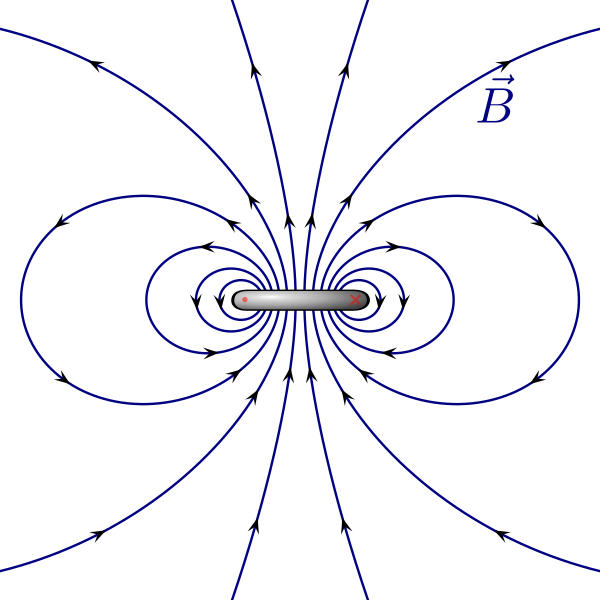
\includegraphics[height=5cm]{fig/fig-campo-magnetico-espira.pdf}\hspace{2cm}
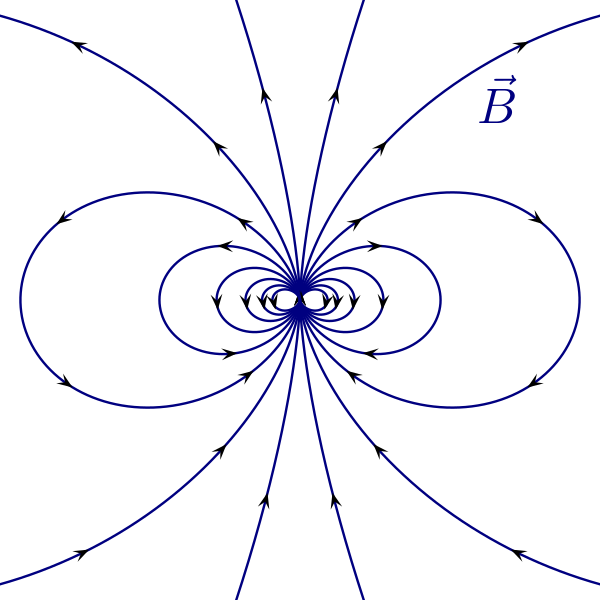
\includegraphics[height=5cm]{fig/fig-campo-dipolo-magnetico.pdf}}
\caption{a) Campo magnético de una espira, b) campo magnético de un dipolo ideal. Adaptadas a partir de \href{http://commons.wikimedia.org/wiki/File:VFPt_dipole_point.svg}{esta} y \href{http://commons.wikimedia.org/wiki/File:VFPt_dipole_magnetic3.svg}{esta} figuras originales.}
\label{fig:dipmag}
\end{figure}

\subsection{Momento dipolar de una espira plana}
\begin{figure}[!h]
\centerline{\includegraphics[height=4cm]{fig/fig-espira-plana-01.pdf}}
\caption{Espira plana y elemento de área.}
\label{fep01}
\end{figure}
En el caso de que la distribución de corriente se concentre en conductores que
describen una curva $\cal C$ (sobre un plano) y transportan corriente $I$, el momento magnético
es dado por
\begin{equation}\label{muintC}
 \vec{\mu}=\frac{I}{2}\oint_{\cal C} \vec{x}\times d\vec{x}.
\end{equation}
En el caso de un \textit{espira plana}, pero de forma arbitraria, tenemos que
(situando el origen en un punto del mismo plano), $\vec{x}\times
d\vec{x}/2=rd\ell_\bot\hat{n}/2=dS\,\hat{n}$, donde $\hat{n}$ es el
vector normal a la espira cuya con dirección dada por la regla de la mano
derecha aplicada a la curva orientada de acuerdo al sentido de circulación de
la corriente\footnote{Equivalentemente, puede obtener este resultado a partir de \eqref{muintC} usando el teorema de Stokes.}. Con esto obtenemos que el momento magnético de una espira plana
de área $A$ es siempre de la forma
\begin{equation}\marginnote{Momento magnético espira plana}
 \boxed{\vec{\mu}=IA\,\hat{n}.}
\end{equation}

\subsection{Relación entre momento magnético y momento angular}
En algunos sistemas se tiene que la densidad de carga eléctrica (en cada
punto) es proporcional a la densidad de masa, de modo que
\begin{equation}
 \rho(x)=\frac{Q}{M} \rho_{\rm m}(x).
\end{equation}
donde $Q$ es la carga total y $M$ la masa total del sistema. Esto ocurre, en
general, en sistemas constituidos por \textit{un sólo tipo de partículas},
masivas y cargadas. En este caso, si cada elemento del sistema se mueve
con velocidad $\vec{v}(x)$, entonces
\begin{equation}
\vec{J}=\rho(x)\vec{v}(x)=\frac{Q}{M} \rho_{\rm m}(x)\vec{v}(x)
\end{equation}
y entonces el momento magnético puede escribirse como
\begin{equation}
 \vec{\mu}=\frac{1}{2}\int_V \vec{x}\times\vec{J}\,dV=\frac{Q}{2M}\int_V
\vec{x}\times\rho_{\rm m}(x)\vec{v}(x)\,dV=\frac{Q}{2M}\int_V
\vec{x}\times d\vec{p},
\end{equation}
donde $d\vec{p}:=\rho_{\rm m}(x)\vec{v}(x)\,dV$ denota el \textbf{momentum lineal} de la masa en el elemento de volumen $dV$. De esta forma $d\vec{L}:=\vec{x}\times d\vec{p}$ es el \textbf{momento angular} del pequeño elemento de masa (respecto al origen elegido) y, finalmente,
\begin{equation}
 \boxed{\vec{\mu}=\frac{Q}{2M}\vec{L}.}
\end{equation}

\section{Fuerza y torque sobre una distribución compacta de corriente}
Consideramos ahora el caso en que una pequeña distribución de corriente
se ubica en una región donde existe un campo magnético \textit{externo}
$\vec{B}(x)$.

La fuerza total que la distribución de corrientes experimenta, debido al campo
externo (es decir, sin tomar en cuenta la autointeracción de la distribución),
es dada por (\ref{fm1}). Para expresar esta fuerza en términos de los momentos multipolares magnéticos de la distribución, situamos nuevamente el
origen de coordenadas en un punto representativo de la distribución y expandimos la
intensidad de campo magnético en puntos dentro de ésta en una serie
de potencias de las componentes del $\vec{x}'$:
\begin{align}
 B_i(\vec{x}+\vec{x}') &= \sum_{n=0}^\infty \frac{1}{n!}x'_{i_1}\cdots x'_{i_n}(\partial_{i_1}\cdots\partial_{i_n}B_i)(x) \label{expB} \\
 &= B_i(x)+x'_j(\partial_jB_i)(x) +
\frac{1}{2}x'_jx'_k(\partial_j\partial_kB_i)(x)+\cdots .
\end{align}
Reemplazando esto en (\ref{fm1}), y tomando en cuenta que la integral sobre la región con corrientes es sobre la variable $\vec{x}'$, encontramos
\begin{align}
F^{\rm m}_i &=  \varepsilon_{ijk}\sum_{n=0}^\infty\frac{1}{n!}M_{i_1\cdots i_nj}(\partial_{i_1}\cdots\partial_{i_n}B_k)(x)\\
&= \varepsilon_{ijk}\left[M_jB_k(x)+M_{lj}(\partial_lB_k)(x)+\frac{1}{2}M_{lnj}(\partial_l\partial_nB_k)(x) +\cdots\right].
\end{align}
Usando (\ref{mmm0}) y (\ref{vmdm}) obtenemos
\begin{eqnarray}
F^{\rm m}_i
&=&\varepsilon_{ijk}\varepsilon_{ljm}\,\mu_m (\partial_lB_k)(x)+\cdots \\
&=& \mu_j(\partial_iB_j)(x)-\mu_i(\partial_jB_j)(x)+\cdots .
\end{eqnarray}
Finalmente, usando la ecuación de campo (\ref{divB}) llegamos a
\begin{equation}
 \boxed{F^{\rm m}_i=\mu_j(\partial_iB_j)(x)+\cdots .}
\end{equation}
En otras palabras, la primera contribución en la expansión multipolar a la
fuerza neta sobre una distribución arbitraria es dada por el término dipolar,
con
\begin{equation}
 \boxed{F_i^{\rm m,(1)}=-\partial_i U_{\rm m}, }
\end{equation}
donde hemos introducido la \textbf{energía de interacción entre un dipolo magnético
y un campo externo}
\begin{equation}
 \boxed{U_{\rm m}(x)=-\vec{\mu}\cdot\vec{B}(x).} \label{Umagdip}
\end{equation}

Similarmente, el torque neto sobre la espira (con respecto al punto de referencia $O$)  puede calcularse a partir de
\begin{equation}
 \tau_i=\varepsilon_{ijk}\int_V x'_j f^{\rm m}_k(x') dV',
\end{equation}
donde $f^{\rm m}_k$ son las componentes de la densidad de fuerza magnética,
definida en (\ref{dfm}). Por lo tanto, usando nuevamente la expansión
(\ref{expB}) podemos escribir,
\begin{eqnarray}
  \tau_i&=&\varepsilon_{ijk}\varepsilon_{kln}\int_V x'_j J_l(x')B_n(x')\, dV' \\
&=&\varepsilon_{ijk}\varepsilon_{kln}\int_V x'_j
J_l(x')\left[B_n(x)+x'_p(\partial_pB_n)_(x) +\cdots\right] dV \\
&=&\varepsilon_{ijk}\varepsilon_{kln}\left[M_{jl}B_n(x)+M_{jpl}(\partial_pB_n)(x)
+\cdots\right] \\
&=&\varepsilon_{ijk}\varepsilon_{kln}\varepsilon_{jlp}\,\mu_pB_n(x)+\cdots\\
&=&\varepsilon_{ijk}\,\mu_jB_k(x)+\cdots 
\end{eqnarray}
o, en notación vectorial
\begin{equation}
 \boxed{\vec{\tau}=\vec{\mu}\times\vec{B}+\cdots .} \label{torqueB}
\end{equation}
Puede verificarse usando (\ref{Umagdip}) y (\ref{torqueB}) que un dipolo
magnético (o, en primera aproximación, toda distribución compacta de
corriente) situado en un campo (homogéneo) externo experimentará un torque
que tenderá a \textit{alinear} el momento magnético de la distribución con el
del campo externo. La posición de equilibrio corresponde al caso en que
$\vec{\mu}$ es paralelo a $\vec{B}$, que es además un equilibrio estable ya
que la energía de interacción es mínima. Más generalmente, el momento
magnético puede realizar un \textbf{movimiento de precesión} en torno al campo
magnético.

%\subsection{Ejemplo: Precesión de Larmor}

\section{Campos magnéticos en la materia}
Análogamente al caso electrostático, en el que un medio se polariza en
presencia de un campo externo, éste puede además \textit{magnetizarse}. Esto
significa que en cada pequeño elemento de volumen (macroscópico) puede existir un momento magnético no nulo. Este momento magnético puede ser producto de
los pequeños ``loops''\, de corrientes inducidas por el campo aplicado sobre los
electrones atómicos. Este tipo de dipolos se inducen en \textit{dirección contraria}
al campo aplicado, por lo que tienden a \textit{reducir} el valor de la inducción
magnética al interior del material. Los materiales \textbf{diamagnéticos} son aquellos en que este tipo de magnetización es dominante. El hecho que las
partículas subatómicas, y en particular los electrones, posean \textit{momentos
magnéticos intrínsecos} (permanentes), hace posible que un material presente
magnetización no nula, de origen distinto a la generada por las corrientes
inducidas. En general, un campo magnético aplicado tenderá a alinear, en
mayor o menor medida, los momentos magnéticos permanentes del material con el campo aplicado, pudiendo compensar y revertir la magnetización debida a las corrientes
inducidas. Los materiales paramagnéticos presentan momentos magnéticos
netos en la misma dirección del campo aplicado. En los ferromagnetos, por
otro lado, la alineación de los momentos magnéticos permanentes es tal que el
momento magnético total es no nulo en ausencia de un campo aplicado, y puede asumir valores varios ordenes de magnitud mayor que el caso de los paramagnetos.

\subsection{Magnetización}
En resumen, consideraremos que en el interior de un medio, existen momentos
magnéticos distribuidos en su interior. Modelaremos esta distribución
definiendo el \textbf{(pseudo-)vector de magnetización} como la densidad de momento
magnético, es decir, como el momento magnético por unidad de volumen en una
pequeña región ($\Delta V\to 0$, desde el punto de vista macroscópico) del
material:
\begin{equation}\marginnote{Definición Magnetización}
\vec{M}(x):= \lim_{\Delta V\to 0} \frac{\Delta \vec{\mu}}{\Delta V}.
\end{equation}
Como consecuencia, la magnetización tiene unidades de corriente por unidad de
longitud: $[\vec{M}]={[\vec{\mu}]}/{L^3}={IL^2}/{L^3}={I}/{L}$.
Con esta definición, tenemos que el momento magnético $d\vec{\mu}(x)$
contenido en un elemento de volumen (macroscópico) $dV$ centrado en un punto con  posición
$\vec{x}$ es
\begin{equation}
d\vec{\mu}(x)=\vec{M}(x)\,dV.
\end{equation}
Entonces, a partir de (\ref{Adip}) podemos calcular al campo (potencial
vectorial) producido por la distribución de momentos dipolares como la
superposición del campo correspondiente al momento dipolar magnético contenido en cada
elemento de volumen:
\begin{eqnarray}
 A_i^{\rm M}(x)&=&\frac{\mu_0}{4\pi}\varepsilon_{ijk}\int_V
\frac{d\mu_j(x')(x_k-x'_k)}{ \left\vert\vec{x} -\vec{x}'\right\vert^3} \\
&=& \frac{\mu_0}{4\pi}\varepsilon_{ijk}\int_V \frac{M_j(x')(x_k-x'_k)}{
\left\vert\vec{x} -\vec{x}'\right\vert^3}dV'.
\end{eqnarray}
Usando la identidad (\ref{id01}) podemos escribir este potencial vectorial
producido por la magnetización del material como:
\begin{eqnarray}
  A_i^{\rm M}(x)&=& \frac{\mu_0}{4\pi}\varepsilon_{ijk}\int_V
M_j(x')\partial'_k\frac{1}{\left\vert\vec{x} -\vec{x}'\right\vert}dV'
\label{AM1}\\
&=& \frac{\mu_0}{4\pi}\varepsilon_{ijk}\int_V\left[\partial'_k\left(
\frac{M_j(x')}{\left\vert\vec{x}
-\vec{x}'\right\vert}\right)-\frac{(\partial'_kM_j(x'))}{\left\vert\vec{x}
-\vec{x}'\right\vert}\right]dV' \\
&=&\frac{\mu_0}{4\pi}\oint_{\partial
V}\frac{\varepsilon_{ijk}M_j(x')}{\left\vert\vec{x}
-\vec{x}'\right\vert}dS'_k+\frac{\mu_0}{4\pi}\int_V\frac{(\varepsilon_{ijk}
\partial'_jM_k(x'))}{ \left\vert\vec{x}-\vec{x}'\right\vert}dV' \\
&=&\frac{\mu_0}{4\pi}\oint_{\partial
V}\frac{(\varepsilon_{ijk}M_j(x')\hat{n}_k)}{\left\vert\vec{x}
-\vec{x}'\right\vert}dS'+\frac{\mu_0}{4\pi}\int_V\frac{(\varepsilon_{ijk}
\partial'_jM_k(x'))}{ \left\vert\vec{x}-\vec{x}'\right\vert}dV'  \\
&=&\frac{\mu_0}{4\pi}\oint_{\partial
V}\frac{j^{\rm M,S}_i(x')}{\left\vert\vec{x}
-\vec{x}'\right\vert}dS'+\frac{\mu_0}{4\pi}\int_V\frac{J^{\rm M}_i(x')}{
\left\vert\vec{x}-\vec{x}'\right\vert}dV'.
\end{eqnarray}
En resumen
\begin{equation}
 \boxed{\vec{A}^{\rm M}(x)=\frac{\mu_0}{4\pi}\int_V\frac{\vec{J}^{\rm M}(x')}{
\left\vert\vec{x}-\vec{x}'\right\vert}dV'+\frac{\mu_0}{4\pi}\oint_{\partial
V}\frac{\vec{j}^{\rm M}(x')}{\left\vert\vec{x}-\vec{x}'\right\vert}dS',}
\label{AM01}
\end{equation}
donde hemos definido la \textbf{densidad de corriente de magnetización}
$\vec{J}^{\rm M}$ y la \textbf{densidad de corriente superficial de
magnetización} $\vec{j}^{\rm M}$ por
\begin{equation}\marginnote{corrientes de magnetización}
\boxed{\vec{J}^{\rm M}(x):=\vec\nabla\times\vec{M}(x), \qquad \vec{j}^{\rm
M}(x):=\vec{M}(x)\times\hat{n}(x).}
\end{equation}
Estas definiciones de densidades de corriente, que pueden ser reales o
ficticias dependiendo del origen de la magnetización $\vec{M}$, son de utilidad
puesto que, de acuerdo a (\ref{AM01}), el campo producido por la magnetización
es \textit{equivalente} al campo producido (a través de la ley de Biot-Savart)
por las corrientes descritas por $\vec{J}^{\rm M}$ en el interior del material y
por $\vec{j}^{\rm M}$ en su superficie.

\begin{figure}[!h]
\centerline{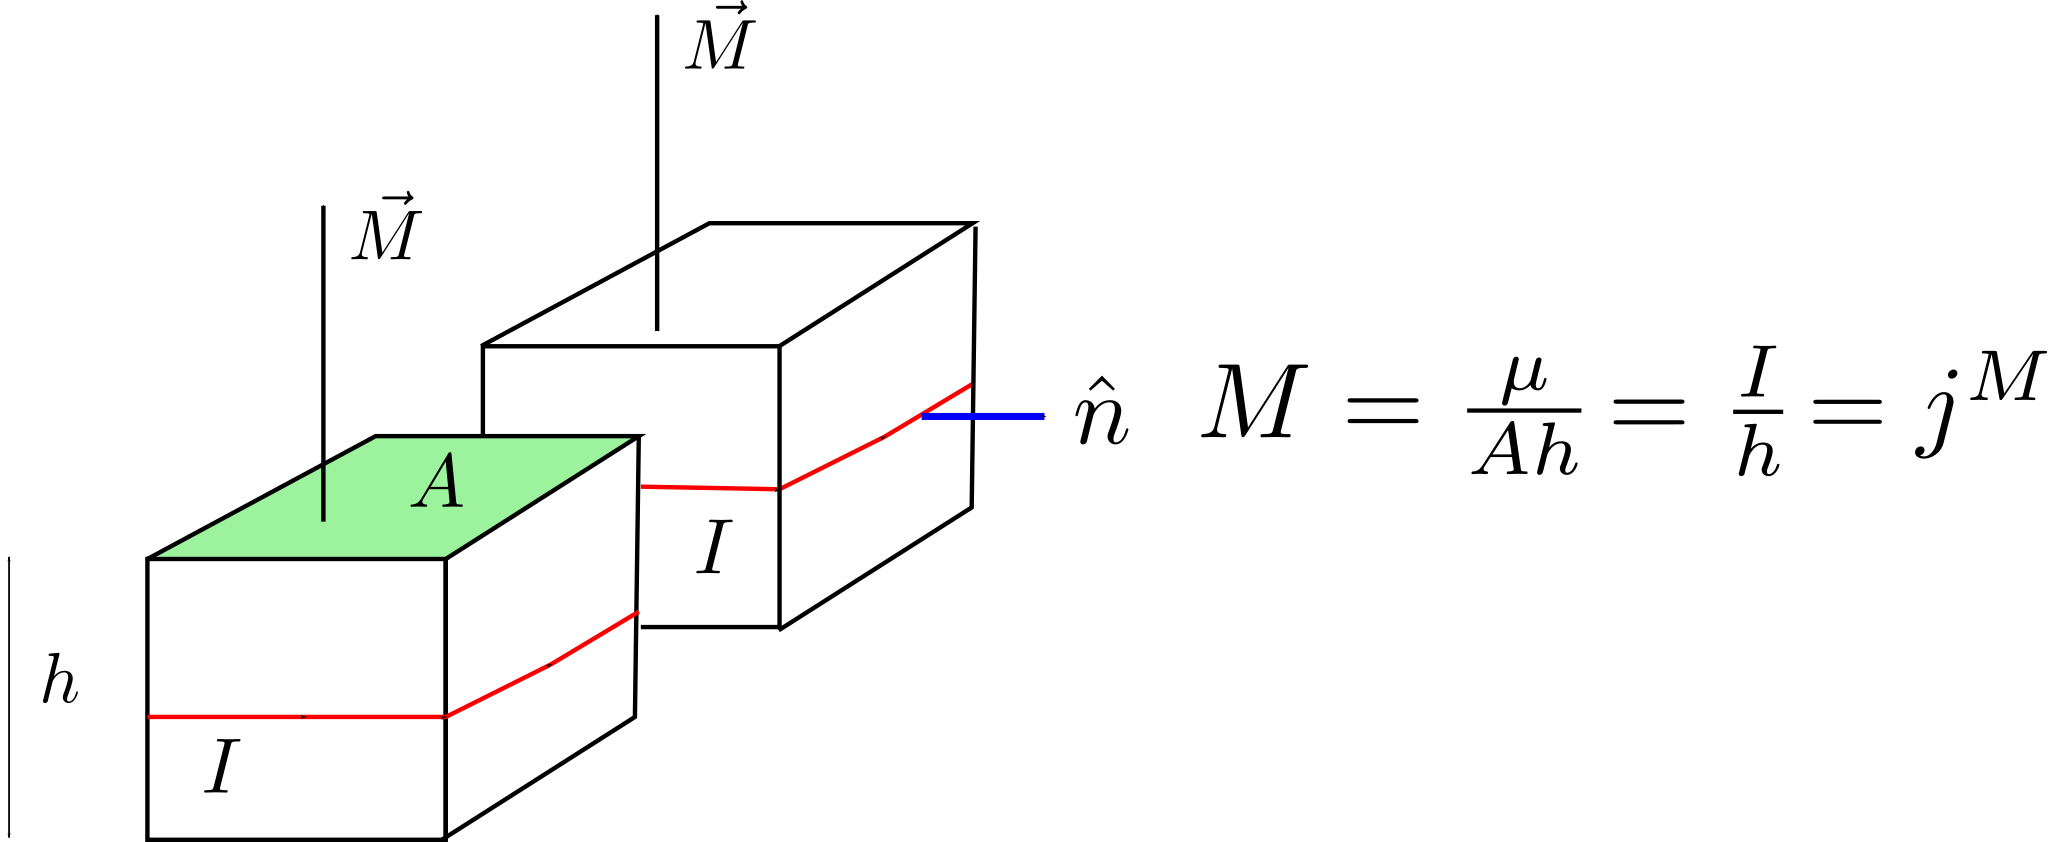
\includegraphics[height=3cm]{fig/fig-corriente-magnetizacion-superficie.pdf}
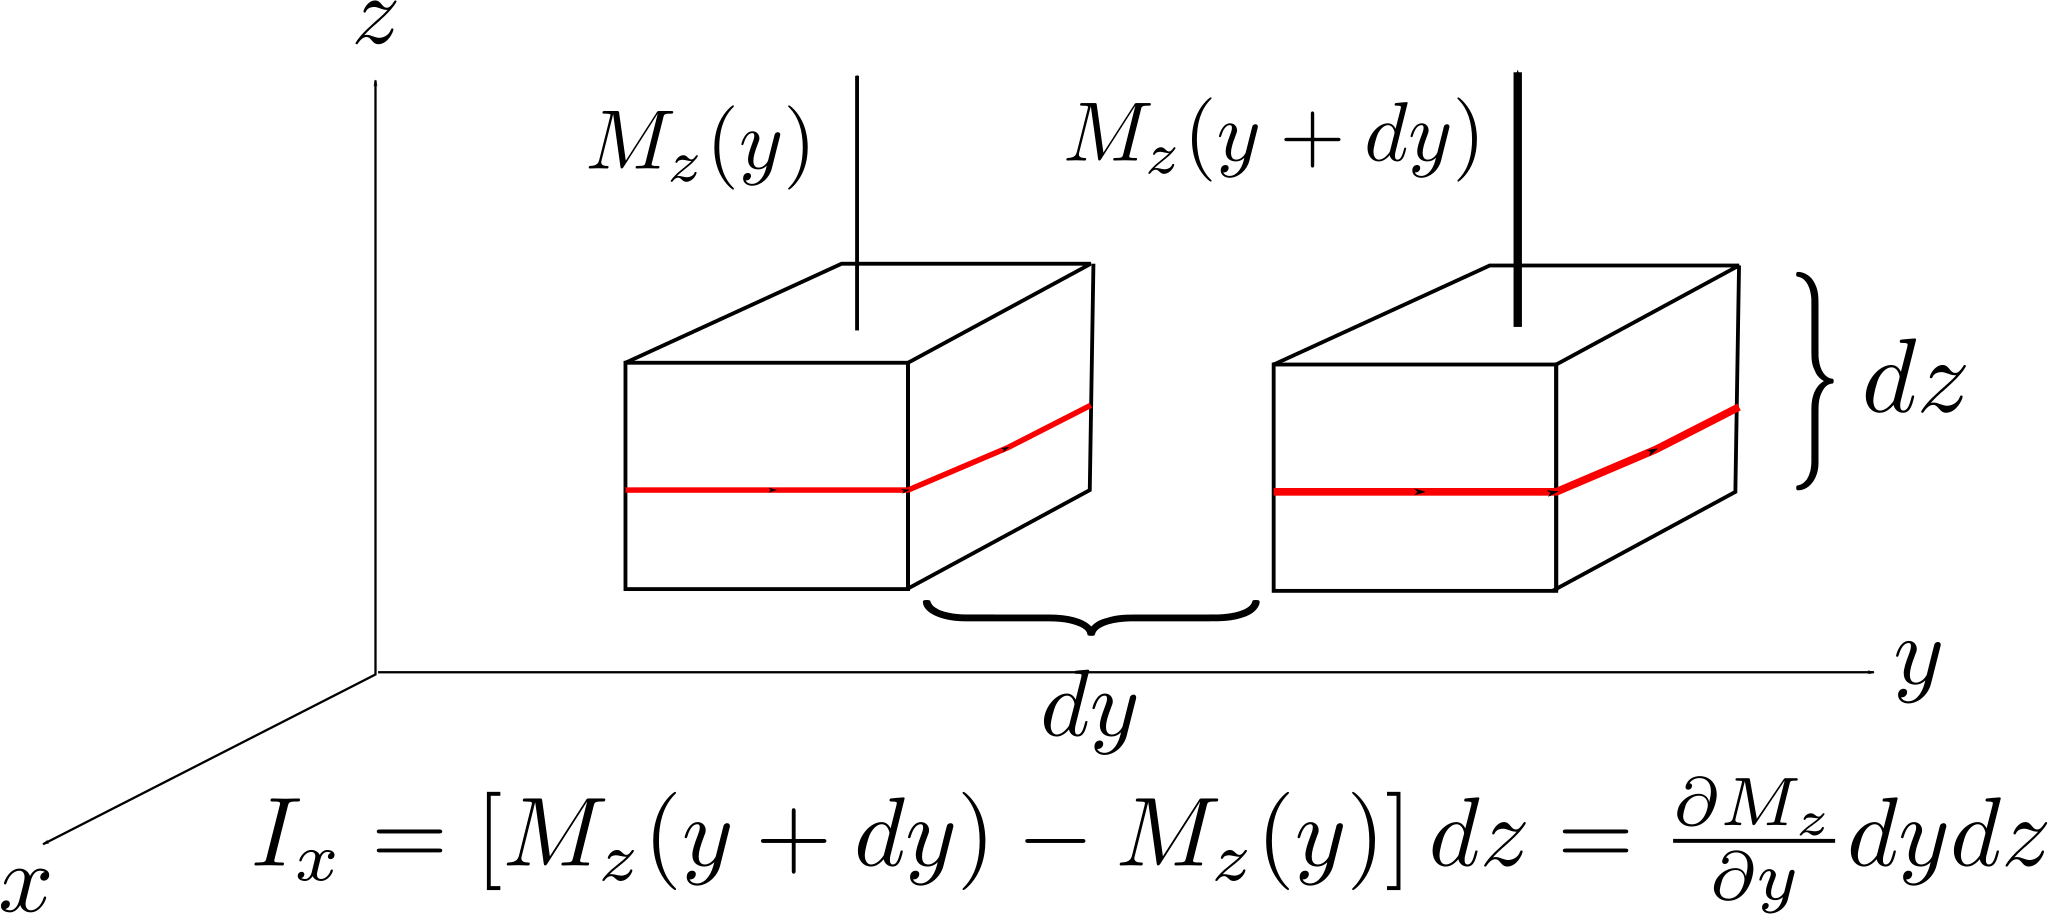
\includegraphics[height=3cm]{fig/fig-corriente-magnetizacion-volumen.pdf}}
\caption{Corrientes de magnetización de volumen y superficie. (Figura original gentileza de A. Maldonado) *** EDITAR, MEJORAR, EXPLICAR ***}
\label{fig-corriente-magnetizacion}
\end{figure}

Usando (\ref{AM1}) podemos calcular la contribución de la magnetización a  la inducción magnética como:
\begin{eqnarray}
 B_i^{\rm M}&=&\varepsilon_{ijk}\partial_jA_k^{\rm M} \\
&=&\frac{\mu_0}{4\pi}\varepsilon_{ijk}\varepsilon_{kln}\int_V
M_l(x')\partial_j\partial'_n\frac{1}{\left\vert\vec{x}
-\vec{x}'\right\vert}dV'\\
&=&-\frac{\mu_0}{4\pi}\left(\delta_{il}\delta_{jn}-\delta_{in}
\delta_{jl}\right)\int_VM_l(x')\partial_j\partial_n\frac{1}{\left\vert\vec{x}
-\vec{x}'\right\vert}dV'\\
&=&\frac{\mu_0}{4\pi}\int_V\left[M_j(x')\partial_j\partial_i\frac{1}{
\left\vert\vec { x }-\vec{x}'\right\vert}-M_i(x')\partial_j\partial_j\frac{1}{
\left\vert\vec { x }-\vec{x}'\right\vert}\right]dV'\\
&=&\frac{\mu_0}{4\pi}\partial_i\left[\int_VM_j(x')\partial_j\frac{1}{
\left\vert\vec{x}-\vec{x}'\right\vert}dV'\right]-\frac{\mu_0}{4\pi}\int_V
M_i(x')\nabla^2\frac{1} {\left\vert\vec {x}-\vec{x}'\right\vert}dV'\\
&=&-\frac{\mu_0}{4\pi}\partial_i\left[\int_VM_j(x')\partial'_j\frac{1}{
\left\vert\vec{x}-\vec{x}'\right\vert}dV'\right]+\mu_0\int_V
M_i(x')\delta^{(3)}(\vec{x}-\vec{x}')dV',
\end{eqnarray}
de donde obtenemos:
\begin{equation}
 \boxed{\vec{B}^{\rm M}(x)=\mu_0\vec{M}(x)-\mu_0\vec\nabla\phi^*_{\rm M}(x),}
\label{BM}
\end{equation}
donde hemos definido el \textbf{potencial escalar de magnetización}\footnote{Note que éste es un campo \textit{distinto} al potencial escalar magnético definido en la sección \ref{secpem}.}
\begin{equation}\marginnote{Potencial escalar de magnetización}
 \boxed{\phi^*_{\rm M}(x):=\frac{1}{4\pi}\int_VM_j(x')\partial'_j\frac{1}{
\left\vert\vec{x}-\vec{x}'\right\vert}dV'=\frac{1}{4\pi}
\int_V\frac{\vec{M}(x')\cdot (\vec{x}-\vec{x}')}{\left\vert\vec{x}-\vec{x}
'\right\vert^3} dV'. }
\end{equation}
En un sistema general existirán, además de la magnetización, corrientes
\textit{externas} (también llamadas \textit{libres} o \textit{de transporte}),
por lo que la inducción magnética total es dada por:
\begin{equation}
 \vec{B}(x)=\vec{B}^{\rm ext}(x)+\vec{B}^{\rm M}(x) .
\end{equation}
Usando (\ref{BS2}) y (\ref{BM}) encontramos finalmente una expresión para 
la inducción magnética macroscópica total en un medio magnetizado y con
corrientes externas:
\begin{equation}\marginnote{$\vec{B}$: corrientes externas + magnetización}
\boxed{ \vec{B}(x)=\frac{\mu_0}{4\pi}\int_V\frac{\vec{J}_{\rm ext}
(x')\times\left(\vec{x}-\vec{x}'\right)}{\left\vert\vec{x}-\vec{x}'\right\vert^3
} dV' +\mu_0\vec{M}(x)-\mu_0\vec\nabla\phi^*_{\rm M}(x).}
\label{BMG}
\end{equation}

\subsection{Excitación magnética}\label{sec:defH}
Al calcular el rotor del campo definido en (\ref{BMG}), vea (\ref{ley-Ampere}),
encontramos:
\begin{equation}
 \vec\nabla\times\vec{B}=\mu_0\,\vec{J}_{\rm ext}
+\mu_0\vec\nabla\times\vec{M}.
\end{equation}
De aquí, podemos escribir
\begin{equation}
 \vec\nabla\times\left(\frac{1}{\mu_0}\vec{B}-\vec{M}\right)=\vec{J}_{
\rm ext}.
\end{equation}
Esto motiva definir la \textbf{excitación magnética} (también llamada
\textbf{intensidad de campo magnético}):
\begin{equation}\marginnote{Excitación magnética}\label{defH}
\boxed{\vec{H}(x):=\frac{1}{\mu_0}\vec{B}(x)-\vec{M}(x),}
\end{equation}
es decir,
\begin{equation}\label{HJM}
\vec{H}(x):=\frac{1}{4\pi}\int_V\frac{\vec{J}_{\rm ext}
(x')\times\left(\vec{x}-\vec{x}'\right)}{\left\vert\vec{x}-\vec{x}'\right\vert^3
} dV' -\vec\nabla\phi^*_{\rm M}(x) ,
\end{equation}
que satisface entonces la ``ley de Amp\`ere'',
\begin{equation}\marginnote{L. de Amp\`ere para $\vec{H}$}
 \boxed{\vec\nabla\times\vec{H}=\vec{J}_{\rm ext}} \label{rotHj}
\end{equation}
o, en su versión integral,
\begin{equation}
 \boxed{\oint_{\cal C}\vec{H}\cdot d\vec\ell=I_{\rm ext} .} \label{intHI}
\end{equation}
Análogamente al caso del vector de desplazamiento eléctrico $\vec{D}$, la
intensidad de campo magnético $\vec{H}$ es una cantidad útil puesto que está
relacionada, a través de la ecuación (\ref{rotHj}), con las corrientes
externas del sistema, que son las corrientes que (en principio) pueden ser
manipuladas.

A partir de (\ref{HJM}) vemos que \textit{en regiones sin corrientes externas}, la excitación magnética puede derivarse íntegramente del potencial escalar de magnetización\footnote{Compare con \eqref{Bgradphi}.},
\begin{equation}\marginnote{Si $\vec{J}_{\rm ext}=\vec{0}$}\label{HpM}
\vec{H}(x)= -\vec\nabla\phi^*_{\rm M}(x).
\end{equation}

\subsection{Condiciones de continuidad en interfaces}
\begin{figure}[!h]
\centerline{\includegraphics[height=5cm]{fig/fig-condicion-borde-magnetica-01.pdf}}
\caption{Condiciones de continuidad para $\vec{H}$ en una interface de dos
medios magnéticos.}
\label{BM1}
\end{figure}
Al aplicar la ley de Amp\`ere (\ref{intHI}) al circuito de la figura \ref{BM1},
y considerando que
\begin{equation}\label{IextjS}
 I_{\rm ext}=\int_S\vec{J}_{\rm ext}\cdot d\vec{S}=\int_S\vec{J}_{\rm ext}\cdot
(\hat{n}\times\hat{t})\,dS=\vec{j}_{\rm ext}\cdot
(\hat{n}\times\hat{t})\,\ell=(\vec{j}_{\rm ext}\times\hat{n})\cdot\hat{t}\,\ell ,
\end{equation}
encontramos
\begin{equation}
 \boxed{\left(\vec{H}_2-\vec{H}_1\right)\cdot\hat{t}=(\vec{j}_{\rm
ext}\times\hat{n})\cdot\hat{t}} \label{Hint}
\end{equation}
o, equivalentemente
\begin{equation}
\boxed{\hat{n}\times\left(\vec{H}_2-\vec{H}_1\right)=\vec{j}_{\rm
ext}.}
\end{equation}
Note que en (\ref{IextjS}) el lado derecho contiene a la \textbf{densidad de corriente superficial externa} $\vec{j}_{\rm ext}$. En este caso puede considerarse que $\vec{J}_{\rm ext}=\vec{j}_{\rm ext}\delta(z)$, donde la superficie que limita las dos regiones está determinada por la condición $z=0$, siendo $z$ una coordenada normal a la superficie.

\textbf{Si no hay corrientes externas de superficie, entonces la componente \textit{tangencial} de la excitación magnética cruza continuamente la interface}. En general, si
existen corrientes externas de superficie, la componente de la intensidad de
campo magnético paralela a $\vec{j}_{\rm ext}=j_{\rm ext}\,\hat{\jmath}$ cruzará continuamente la interface, mientras que la componente ortogonal tendrá una discontinuidad de magnitud $j_{\rm ext}$. Esto puede verse directamente
de (\ref{Hint}) eligiendo $\hat{t}$ en la dirección y sentido de
$\vec{j}_{\rm ext}$, es decir, $\hat{t}=\hat{\jmath}$, obteniendo
\begin{equation}
 H_2^\parallel=H_1^\parallel,  \qquad H^\parallel:=\vec{H}\cdot\hat{\jmath},
\end{equation}
mientras que, eligiendo $\hat{t}=\hat{\jmath}\times\hat{n}$, encontramos
\begin{equation}
 H_2^\perp-H_1^\perp=j_{ext},  \qquad
H^\perp:=\vec{H}\cdot(\hat{\jmath}\times\hat{n}).
\end{equation}

Estas relaciones se complementan con aquella que se desprende del hecho que el campo magnético tiene siempre divergencia nula (independientemente del medio considerado). Análogamente al caso eléctrico, ver por ejemplo \eqref{saltoDn}, la ecuación \eqref{divB} implica 
\begin{equation}\label{saltoBn}
\boxed{\left(\vec{B_2}-\vec{B_1}\right)\cdot\hat{n}=0,}
\end{equation}
es decir, la componente de $\vec{B}$ normal a la superficie es continua en la interface.

\subsection{Relación constitutiva, susceptibilidad magnética}
Análogamente al caso electrostático, se llama relación constitutiva a la
relación entre la magnetización de un material (la ``respuesta'' de éste)
con el campo magnético existente, por ejemplo:
\begin{equation}
 \vec{M}=\vec{M}[\vec{H}].
\end{equation}
Esta relación puede ser no-local, no-lineal, anisótropa e inhomogénea, y es usualmente inferida a partir de experimentos. Sin
embargo, muchos materiales pueden ser descritos por relaciones \textit{locales}. En
este caso puede parametrizarse la dependencia de la magnetización con la
intensidad magnética por medio de una serie de la forma
\begin{equation}
M_i(x)=M_i(H_j(x))=\left.M_i\right|_{\vec{H}=\vec{0}}
+\chi^{\rm m}_{ij}(x)H_j(x)+\chi^{\rm m}_{ijk}(x)H_j(x)H_k(x)+\cdots.
\end{equation}
%\begin{equation}
%M_i(x)=M_i(H_j(x))=\left.M_i\right|_{\vec{H}=\vec{0}}
%+H_j\left(\partial_jM_i\right)_{\vec{H}=\vec{0}}+\frac{1}{2}
%H_jH_k\left(\partial_j\partial_k M_i\right)_{\vec{H}=\vec{0}}+\cdots.
%\end{equation}
Para medios locales, \textit{lineales} y \textit{sin magnetización permanente}
($\left.M_i\right|_{\vec{H}=\vec{0}}=0$), la relación se reduce a
\begin{equation}
 \boxed{M_i(x)=\chi^{\rm m}_{ij}(x)H_j(x),}
\end{equation}
donde $\chi^{\rm m}_{ij}$ es el \textbf{tensor de susceptibilidad magnética} del
material. En este caso, la inducción magnética adopta la forma
\begin{equation}
 \boxed{B_i(x)=\mu_{ij}(x)H_j(x)=\mu_0\,\kappa^{\rm m}_{ij}(x)H_j(x),}
\end{equation}
con el tensor de \textbf{permeabilidad magnética} $\mu_{ij}$ y el
tensor de \textbf{permeabilidad relativa} $\kappa^{\rm m}_{ij}$, definidos por
\begin{equation}
 \boxed{\mu_{ij}:=\mu_0\left(\delta_{ij}+\chi^{\rm
m}_{ij}\right)=\mu_0\kappa^{\rm m}_{ij}.}
\end{equation}
Finalmente, en el caso de medios locales, lineales e isótropos, las
expresiones anteriores para la relación constitutiva se reducen a
\begin{equation}
 \vec{M}(x)=\chi_{\rm m}(x)\vec{H}(x),
\end{equation}
\begin{equation}
 \vec{B}(x)=\mu(x)\vec{H}(x)=\mu_0\,\kappa_{\rm m}(x)\vec{H}(x),
\end{equation}
\begin{equation}
 \mu:=\mu_0\left(1+\chi_{\rm m}\right)=\mu_0\kappa_{\rm m}.
\end{equation}


\subsubsection{Ecuación de Laplace para el potencial escalar de magnetización}
Como vimos en la sección \ref{sec:defH}, \textit{en regiones libres de corrientes externas} la excitación magnética $\vec{H}$ es propocional al gradiente del potencial escalar de magnetización, ver (\ref{HpM}). Si además el medio es \textit{lineal e isótropo}, entonces $\vec{B}=\mu\vec{H}=-\mu\vec{\nabla}\phi^\ast_{\rm M}$. Finalmente, si además el medio es \textit{homogéneo}, encontramos, usando (\ref{divB}), que el potencial escalar de magnetización satisface la ecuación de Laplace,
\begin{equation}
\nabla^2\phi^\ast_{\rm M}=0.
\end{equation}


\subsection{Paramagnetismo, diamagnetismo, ferromagnetismo}

\subsubsection{Diamagnetismo}
En este tipo de materiales $\vec{M}$ \textbf{tiene dirección opuesta a}  $\vec{H}$, por lo que $\chi_{\rm m}<0$ y $\kappa_{\rm m}<1$ y la inducción magnética $\vec{B}$ es \textbf{debilitada} (respecto al valor que asumiría en el vacío, dada la misma distribución de corrientes externas). Este tipo de materiales requiere que no existan \textit{momentos magnéticos permanentes} significativos, de modo que la magnetización se deba principalmente a \textbf{corrientes inducidas}. Estas \textbf{corrientes inducidas generan momentos dipolares en sentido contrario al campo que las induce}, por lo que \textbf{la inducción magnética disminuye en el interior de un diamagneto}. En la mayoría de los casos de diamagnetismo la susceptibilidad magnética es independiente de la
temperatura y posee un valor muy pequeño: $|\chi_{\rm m}|\lesssim 10^{-5}$. El
diamagnetismo es una propiedad general, es decir, que se presenta en todos los
materiales (siempre se producen pequeñas corrientes inducidas), pero se dice
que un material es diamagnético si este efecto es el dominante, es decir,
cuando no existen otras fuentes de magnetización que reviertan la contribución diamagnética.
Ejemplos de materiales diamagnéticos: casi todas las substancias orgánicas,
metales nobles (oro, plata, cobre, mercurio, ...). Un caso extremo de
diamagnetismo es un \textbf{superconductor}, en el que la inducción magnética
es \textbf{anulada en su interior}, $\chi_{\rm m}=-1$ y $\kappa_{\rm m}=0$ (``diamagneto ideal'').

\subsubsection{Paramagnetismo}
 En este tipo de materiales la magnetización $\vec{M}$
tiene la misma dirección y sentido que $\vec{H}$. Equivalentemente $\vec{M}$
tiene la misma dirección y sentido que $\vec{B}$, de modo que
$\chi_{\rm m}>0$, $\kappa_{\rm m}>1$. Por esto, en un material paramagnético la inducción magnética $\vec{B}$ es \textbf{reforzada}. Este caso requiere que el material posea \textit{momentos magnéticos permanentes}, que puedan anilearse con el campo magnético.
A la tendencia de los momentos magnéticos a alinearse se
contrapone el ``desorden'' relacionado con las agitaciones térmicas del
material. Por esto, \textbf{en un material paramagnético $\chi_{\rm}$ disminuye a
medida que la temperatura aumenta}. Muchos materiales paramagnéticos satisfacen
la \textbf{ley de Curie}: $\chi_{\rm}\propto 1/T$.
\begin{table}[h!]
\begin{center}
\begin{tabular}{c|c}
Material & $\chi_{\rm m}$ \\ \hline\hline
Aluminio & $2,1\times 10^{-5}$ \\
Cobre & $-0,98\times 10^{-5}$ \\
Oro & $-3,5\times 10^{-5}$ \\
Magnesio & $1.2\times 10^{-5}$ \\
Mercurio & $-2,8\times 10^{-5}$ \\
Plata & $-2,4\times 10^{-5}$ \\
Sodio & $0.84\times 10^{-5}$ \\
Titanio & $18.0\times 10^{-5}$ \\
Tungsteno & $7.6\times 10^{-5}$ \\
Hidrógeno (1 atm) & $-0,22\times 10^{-8}$ \\
Nitrógeno (1 atm) & $-0,67\times 10^{-8}$ \\
Oxígeno (1 atm) & $193,5\times 10^{-8}$
\end{tabular}
\caption{Algunos materiales y sus susceptibilidades magnéticas, a temperatura ambiente (Reitz-Milford).}
\end{center}
\end{table}

\subsubsection{Ferromagnetismo}

 En este tipo de materiales (típicamente materiales que
contienen Fierro, Cobalto o Níquel) \textbf{la magnetización no es
proporcional a la excitación magnética}. Esto es algunas veces expresado
diciendo que la \textbf{susceptibilidad magnética efectiva} $\chi_{\rm m}:=M/H$ depende del valor del campo (y de otras variables, como por ejemplo de la temperatura), $\chi_{\rm m}=\chi_{\rm m}(T,\vec{H})$. El ferromagnetismo
requiere también que el material posea dipolos magnéticos permanentes. Debido
a interacciones cuánticas, los momentos magnéticos de un ferromagneto se
ordenan \textit{espontáneamente} (es decir, sin necesidad de campo magnético
externo), cuando la temperatura baja de un cierto valor crítico, llamada
temperatura de Curie, $T_{\rm C}$. En el cero absoluto de temperatura, todos los
momentos magnéticos estarían alineados. A medida que la temperatura aumenta, el
desorden inducido por las vibraciones térmicas tiende a disminuir la
alineación, pero sin conseguir
anular la magnetización total. Cuando la temperatura cruza la temperatura de
Curie, el sistema experimenta una transición de fase, y a partir de ese
momento se comporta como un paramagneto usual.
\begin{table}[h!]
\begin{center}
\begin{tabular}{c||c|c|c|c|c|c}
Material & Fe & Co & Ni & Gd & EuO & CrBr${}_3$  \\ \hline
$T_{\rm C}$ [K] & 1043 & 1393 & 631 & 290 & 69 & 37
\end{tabular}
\caption{Algunos materiales ferromagnéticos y sus temperaturas de Curie 
\cite{Nolting}.}
\end{center}
\end{table}

Típicamente, los ferromagnetos poseen susceptibilidades
magnéticas muy altas y \textbf{la magnetización que presentan depende de
su historia}, es decir, de cómo hayan sido expuestos a campos externos. En
otras palabras, \textbf{dado un valor de la excitación $\vec{H}$ el valor de $\vec{M}$
no es único, sino que depende de cómo se haya alcanzado el valor $\vec{H}$}.
Este fenómeno es conocido como \textbf{histéresis}. El comportamiento de
histéresis típico de un ferromagneto es ilustrado en la figura
\ref{fig-histeresis}.
\begin{figure}[!h]
\centerline{\includegraphics[height=6cm]{fig/fig-histeresis-01.pdf}}
\caption{Curva de histéresis típica para un material ferromagnético.}
\label{fig-histeresis}
\end{figure}
Un material ferromagnético sin magnetización previa sometido a un campo $H$
se magnetiza siguiendo la curva I, llegando a una magnetización máxima $M_S$ (``magnetización de saturación"). 
Si luego se disminuye la intensidad de campo magnético el sistema se comienza
a demagnetizar, pero siguiendo la curva II, de modo que, incluso cuando el
campo $H$ es cero, el material conserva una magnetización no nula (magneto
permanente), llamada ``magnetización remanente''. Esta magnetización puede
ser anulada aplicando un campo en sentido inverso (intensidad de campo
``coercitivo''). La propiedad de histéresis está relacionada con la existencia
de \textbf{dominios magnéticos}, que poseen un momento magnético macroscópico
no nulo y que requieren de energía para reorientarse. La histéresis de los
ferromagnetos es usada en la fabricación de \textbf{dispositivos de memoria}, en los
que la información es codificada en la orientación del momento magnético de
los dominios, que permanece indefinidamente hasta que campos externos sean
usados para cambiar su estado.